%% V1.0
%% 2019/01/16
%% This is the template for a Lab report following an IEEE paper. Modified by Francisco Tovar after Michael Sheel original document.

%% This is a skeleton file demonstrating the use of IEEEtran.cls
%% (requires IEEEtran.cls version 1.8b or later) with an IEEE
%% journal paper.
%%
%% Support sites:
%% http://www.michaelshell.org/tex/ieeetran/
%% http://www.ctan.org/pkg/ieeetran
%% and
%% http://www.ieee.org/


\documentclass[journal]{IEEEtran}

% *** CITATION PACKAGES ***
\usepackage[style=ieee]{biblatex} 
\usepackage[spanish]{babel}
\bibliography{references.bib}    %your file created using JabRef

% *** MATH PACKAGES ***
\usepackage{amsmath}
\usepackage{listings}
\usepackage{xcolor}
\lstset{
    backgroundcolor=\color{lightgray},   % Background color for code
    basicstyle=\ttfamily\footnotesize,     % Font style and size
    keywordstyle=\color{blue},             % Color for keywords
    commentstyle=\color{green},            % Color for comments
    stringstyle=\color{red},               % Color for strings
    numbers=left,                          % Line numbers on the left
    numberstyle=\tiny\color{gray},         % Style for line numbers
    stepnumber=1,                          % Show line numbers every 1 line
    numbersep=5pt,                         % Distance between line numbers and code
    showstringspaces=false                 % Don't show spaces in strings
}

% *** PDF, URL AND HYPERLINK PACKAGES ***
\usepackage{url}
% correct bad hyphenation here
\hyphenation{op-tical net-works semi-conduc-tor}
\usepackage{graphicx}  %needed to include png, eps figures
\usepackage{float}  % used to fix location of images i.e.\begin{figure}[H]

\begin{document}

% paper title
\title{Avance de proyecto: Street View House Numbers (SVHN)}

% author names 
\author {Braulio Isaac Martínez Aceves 747200
        }% <-this % stops a space
        
% The report headers
\markboth{MSC1007A Aprendizaje Automático, Avance de Proyecto, 5 noviembre 2024}%do not delete next lines
{Shell \MakeLowercase{\textit{et al.}}: Bare Demo of IEEEtran.cls for IEEE Journals}

% make the title area
\maketitle

%\begin{IEEEkeywords}
%keywords, temperature, xxxx equation, etc.
%\end{IEEEkeywords}

\section{Introducción y justificación}
% Here we have the typical use of a "W" for an initial drop letter
% and "RITE" in caps to complete the first word.
% You must have at least 2 lines in the paragraph with the drop letter
% (should never be an issue)

El dataset SVHN representa dígitos en imágenes naturales que provienen de fotografías de casas. Detectar y leer texto en fotografías represnta un problema complicado en la disciplina de visión por computadora. Si bien algunos problemas de reconocimiento de caracteres bien delimitados se encuentran resueltos(OCR, reconocimiento de dígitos escritos a mano), el reconocimiento en escenas o imágenes naturales representa un reto mayor debido a los artefactos, ruido o distractores naturales.\cite{svhn} Estas características presentan al dataset como un buen candidato para temas de machine learning.

\section{Objectivos}
\begin{itemize}
        \item Obtención de datos
        \item Preprocesamiento y Feature Engineering
        \item Selección de modelos
        \item Cross-Validation
        \item Entrenamiento y evaluación
\end{itemize}


\subsection{Obtención de datos}
El dataset se obtuvo directamente de HugginFace.\cite{huggingface_svhn}
\begin{lstlisting}[language=Python]
from datasets import load_dataset
ds = load_dataset("ufldl-stanford/svhn",
                  "cropped_digits"
                 )
\end{lstlisting}


\subsection{Preprocesamiento y Feature Engineering}
Debido a la complejidad del problema (dígitos en imágenes naturales a color y con distractores), es de vital importancia realizar el correcto pre-procesamiento y Feature Engineering para facilitar la tarea y rendimiento de nuestro algoritmo predictivo. Como objetivo final se busca reconocer dígitos centrados en imágenes de 32x32, como primera aproximación, se transforma y reduce la imagen a color original a bordes. Para esto, se propone la siguiente lista ordenada de pasos o transformaciones a realizar en cada muestra antes de realizar cualquier entrenamiento:

\begin{enumerate}
        \item Escala de grises: Reducción de 3 canales (RGB) a 1 canal
        \item Sharpening: Mejorar la claridad de la imagen para poder extraer más características
        \item CLAHE: Contrast Limited Adaptive Histogram Equalization, usado para mejorar el contraste de la imagen y reducir ruido
        \item Transformación logarítmica o con mediana: Normalizar los datos para evitar que valores poco comunes (outliers) afecten el entrenamiento
        \item Binary Dynamic Thresholding: Reducir el espacio de escala de grises a [0, 1]
        \item Extracción de contorno: Obtener y mantener sólo los pixeles de contornos de dígitos
        \item Filtro Gaussiano: Reducir el impacto de posibles distractores a los bordes de la imagen
        \item Flattening: Se convierten las imágenes 2D de 32x32 a un solo vector 1D de 1024 elementos
\end{enumerate}

\subsubsection{Visualización de Transformaciones, dígito 7}
En la siguiente secuencia de imágenes se puede observar, paso a paso, las transformaciones a una muestra.

\begin{figure}[H]
        \centering
        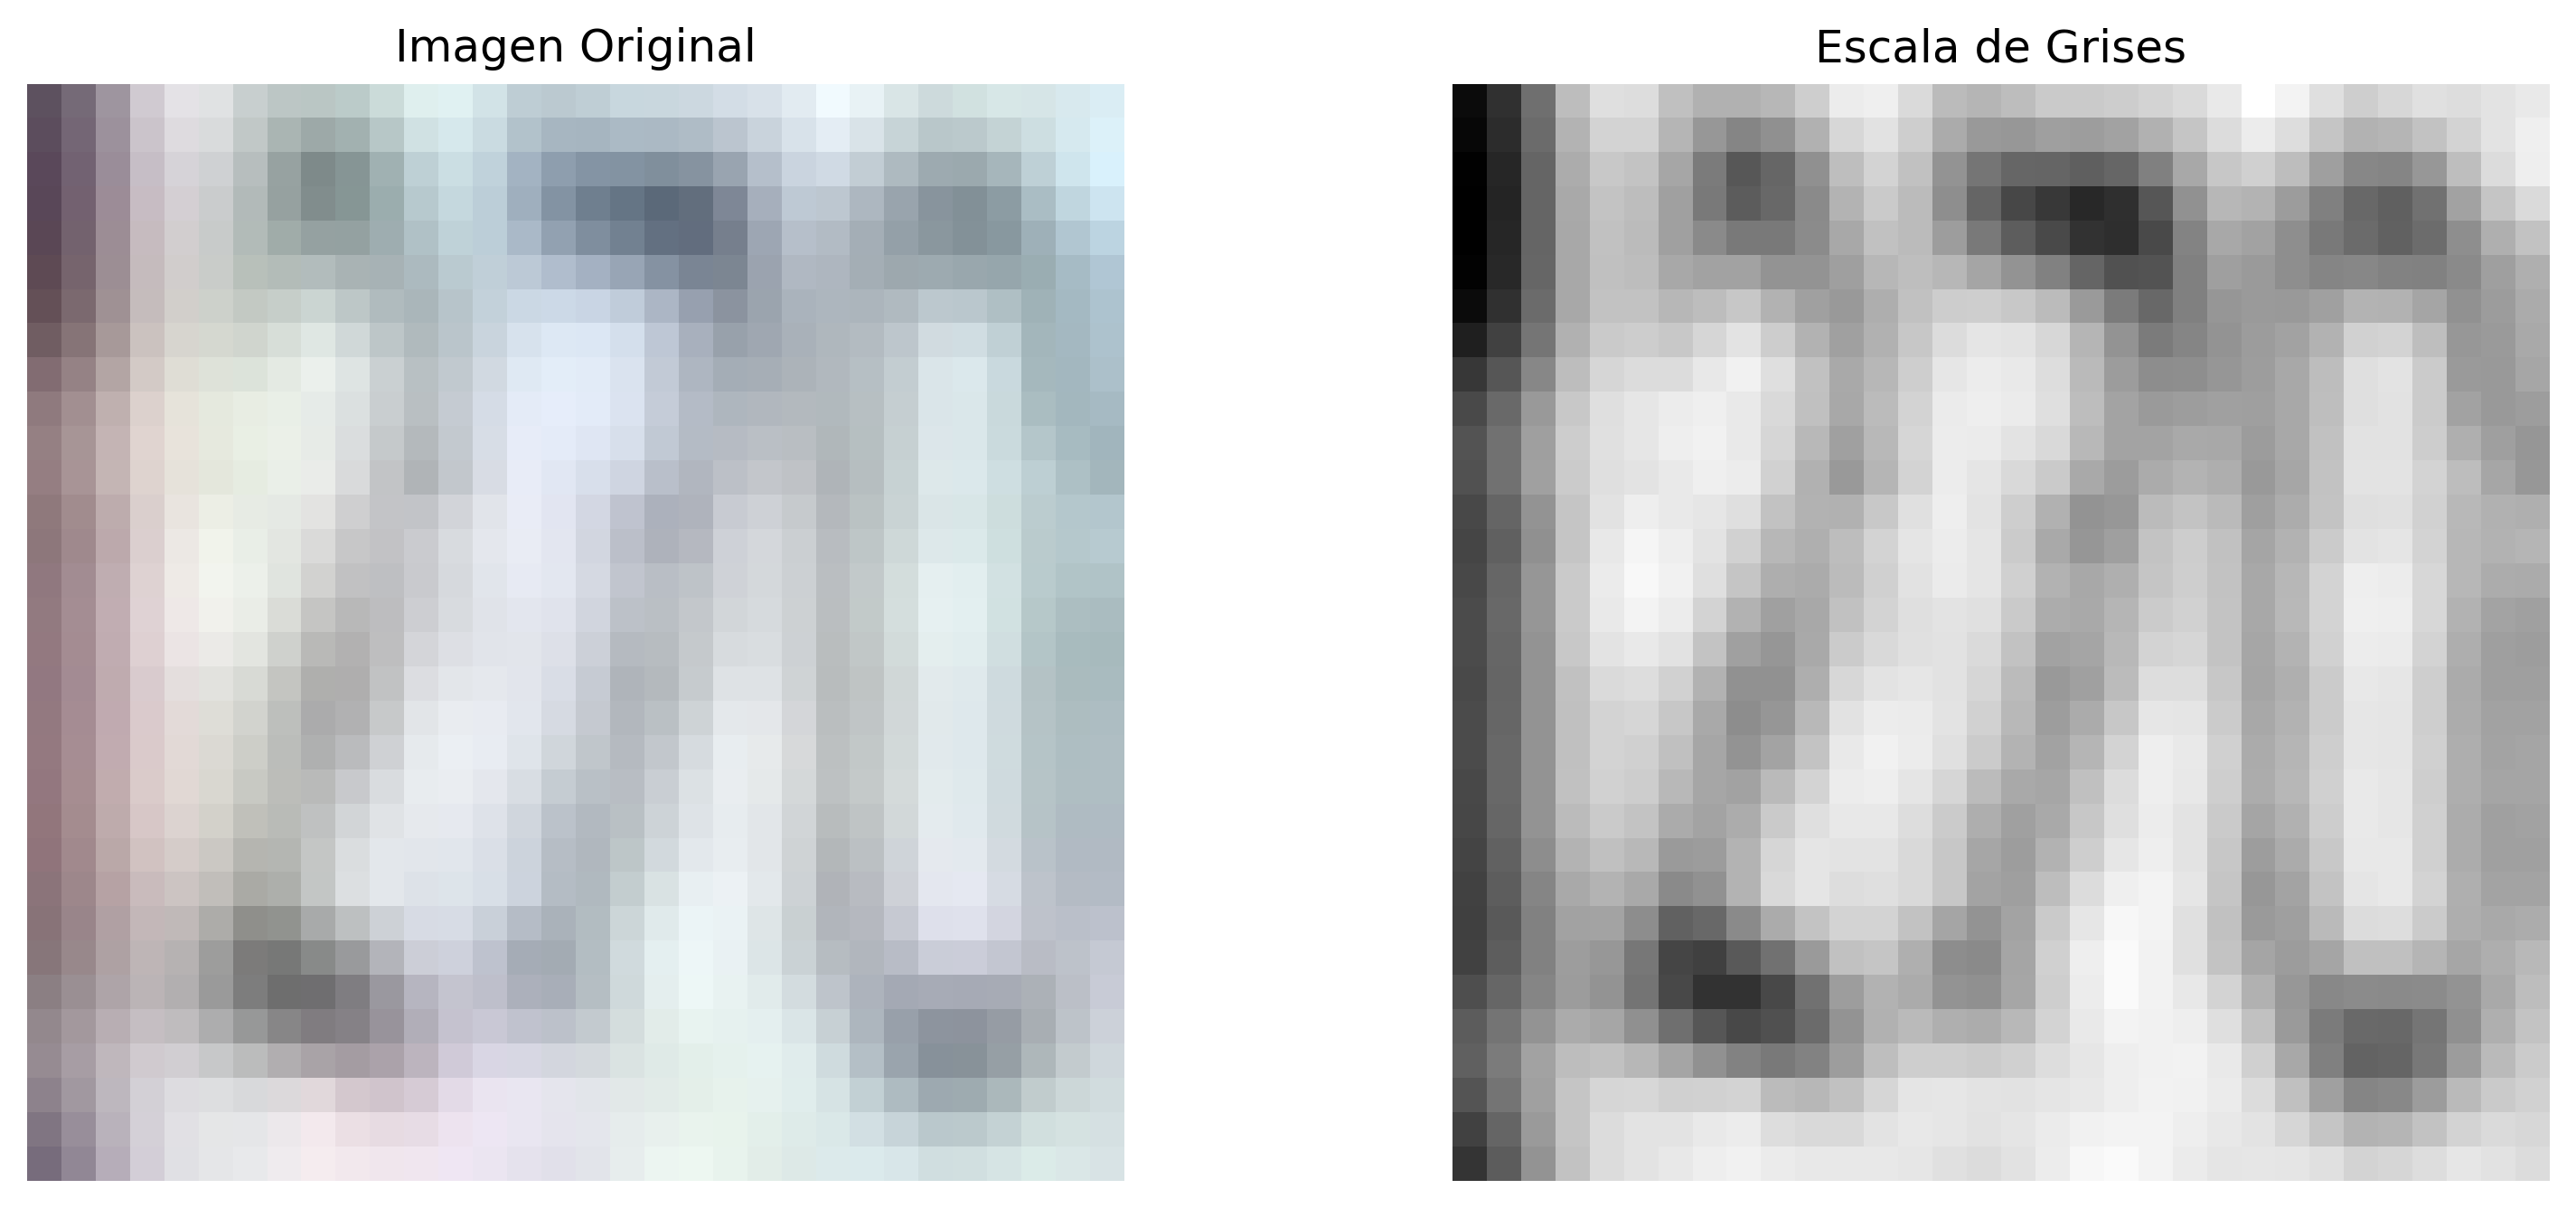
\includegraphics[width=\linewidth]{figures/row_1_images.png}
        \caption{Imagen original y transformación a escala de grises}
        \label{fig:row_1}
\end{figure}

\begin{figure}[H]
        \centering
        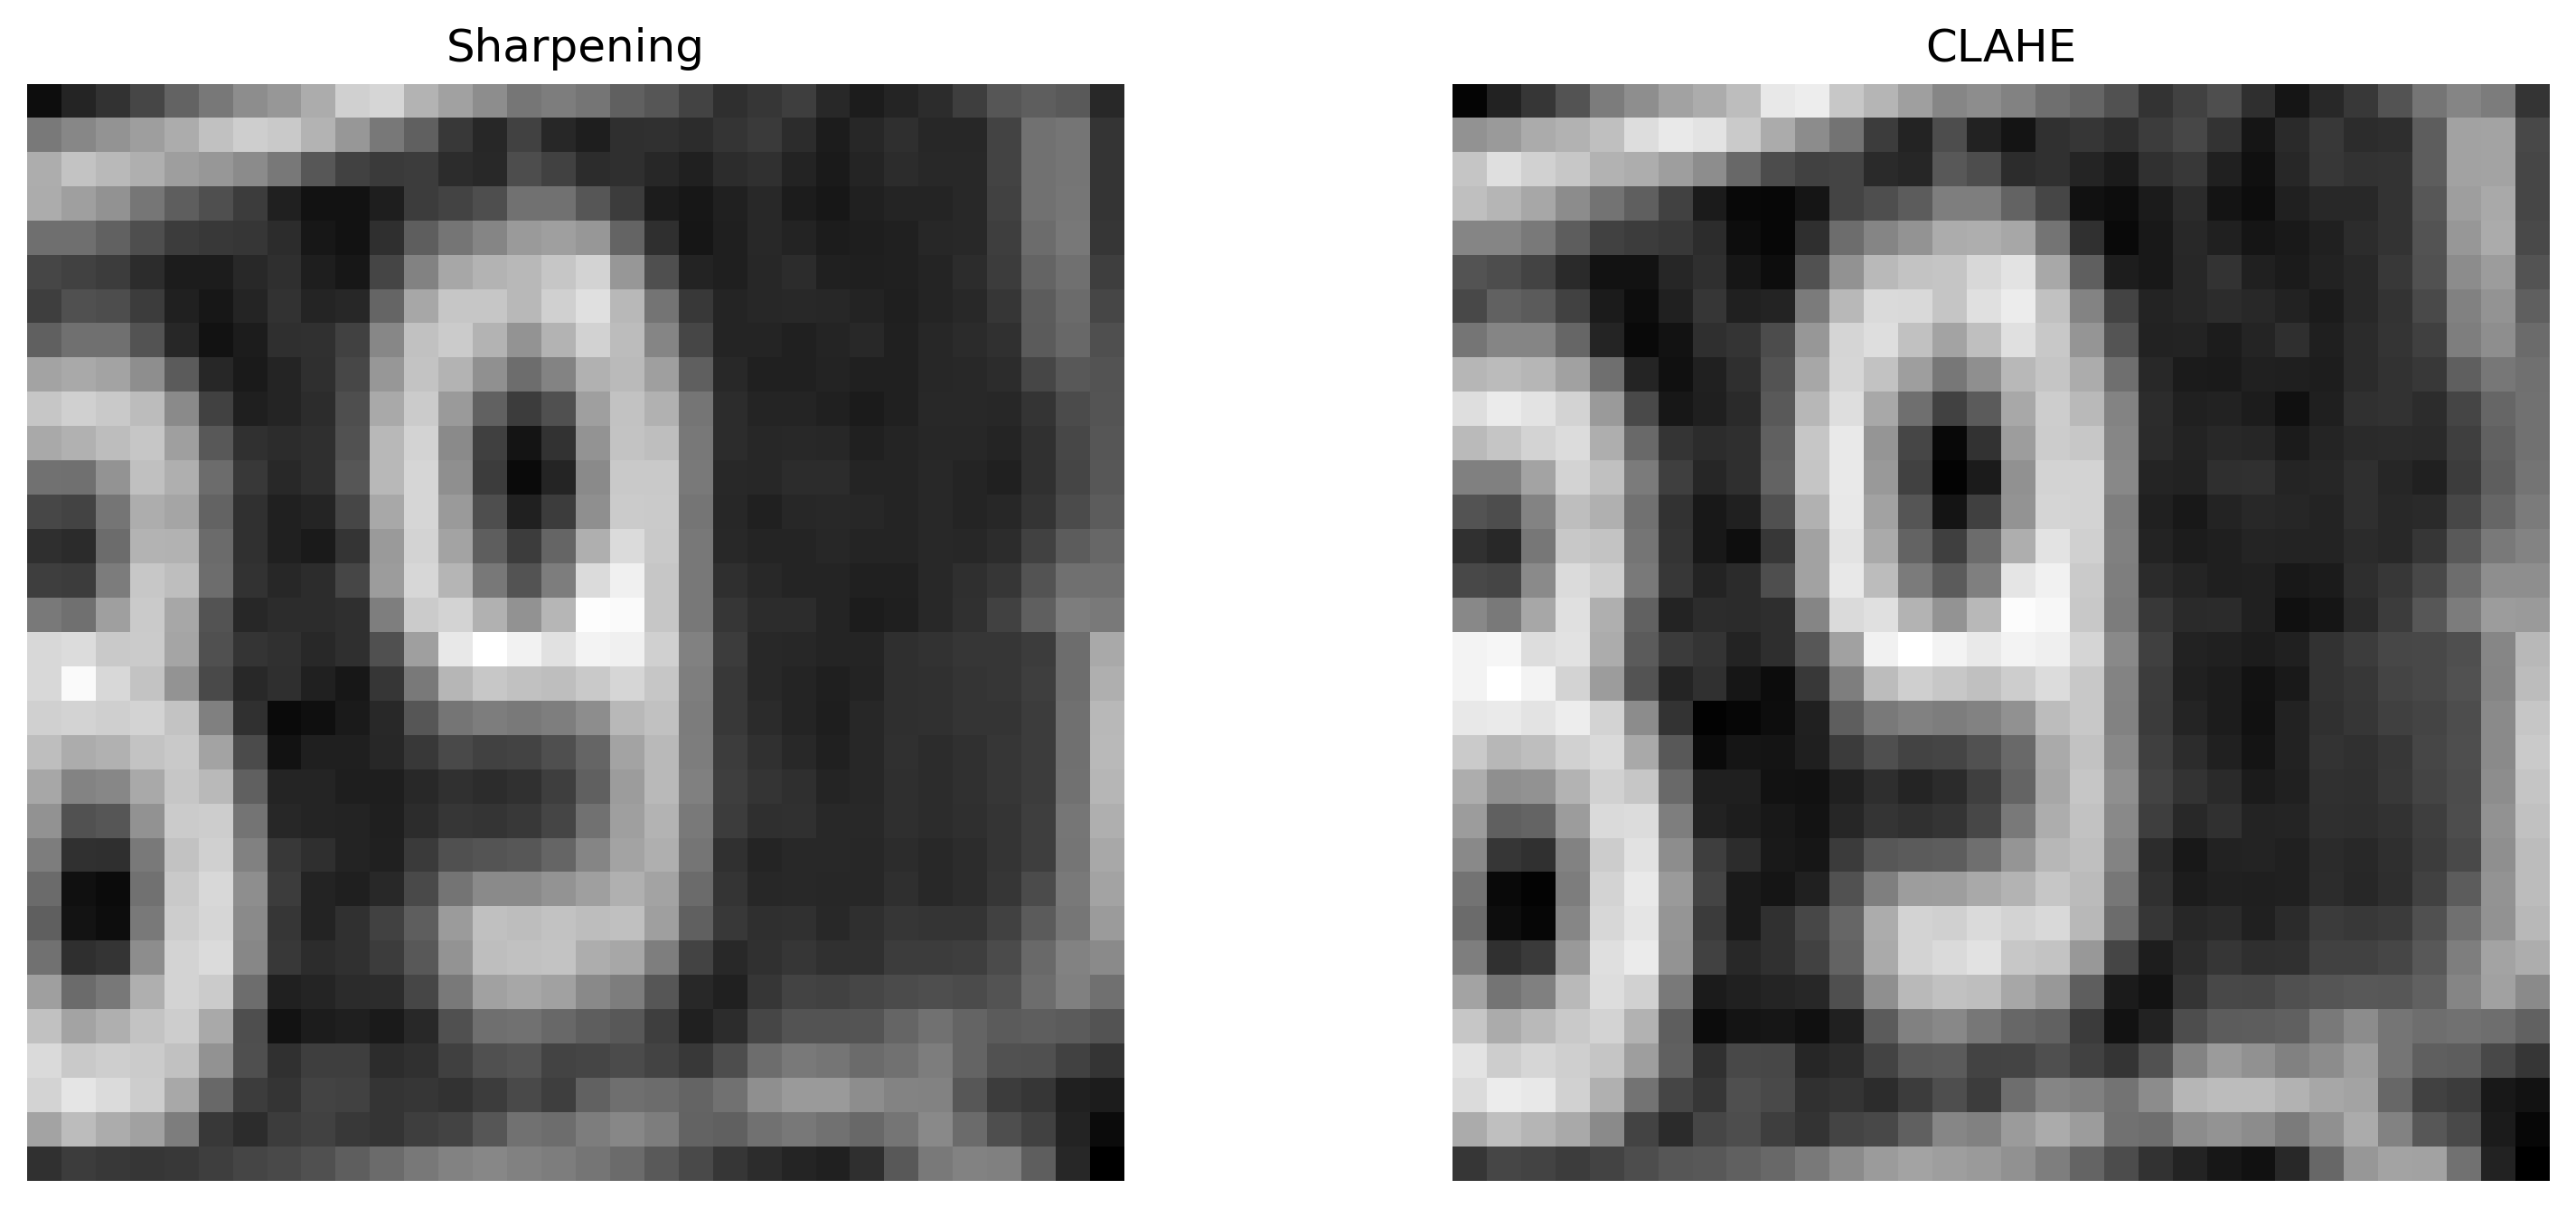
\includegraphics[width=\linewidth]{figures/row_2_images.png}
        \caption{Sharpening y CLAHE}
        \label{fig:row_2}
\end{figure}

\begin{figure}[H]
        \centering
        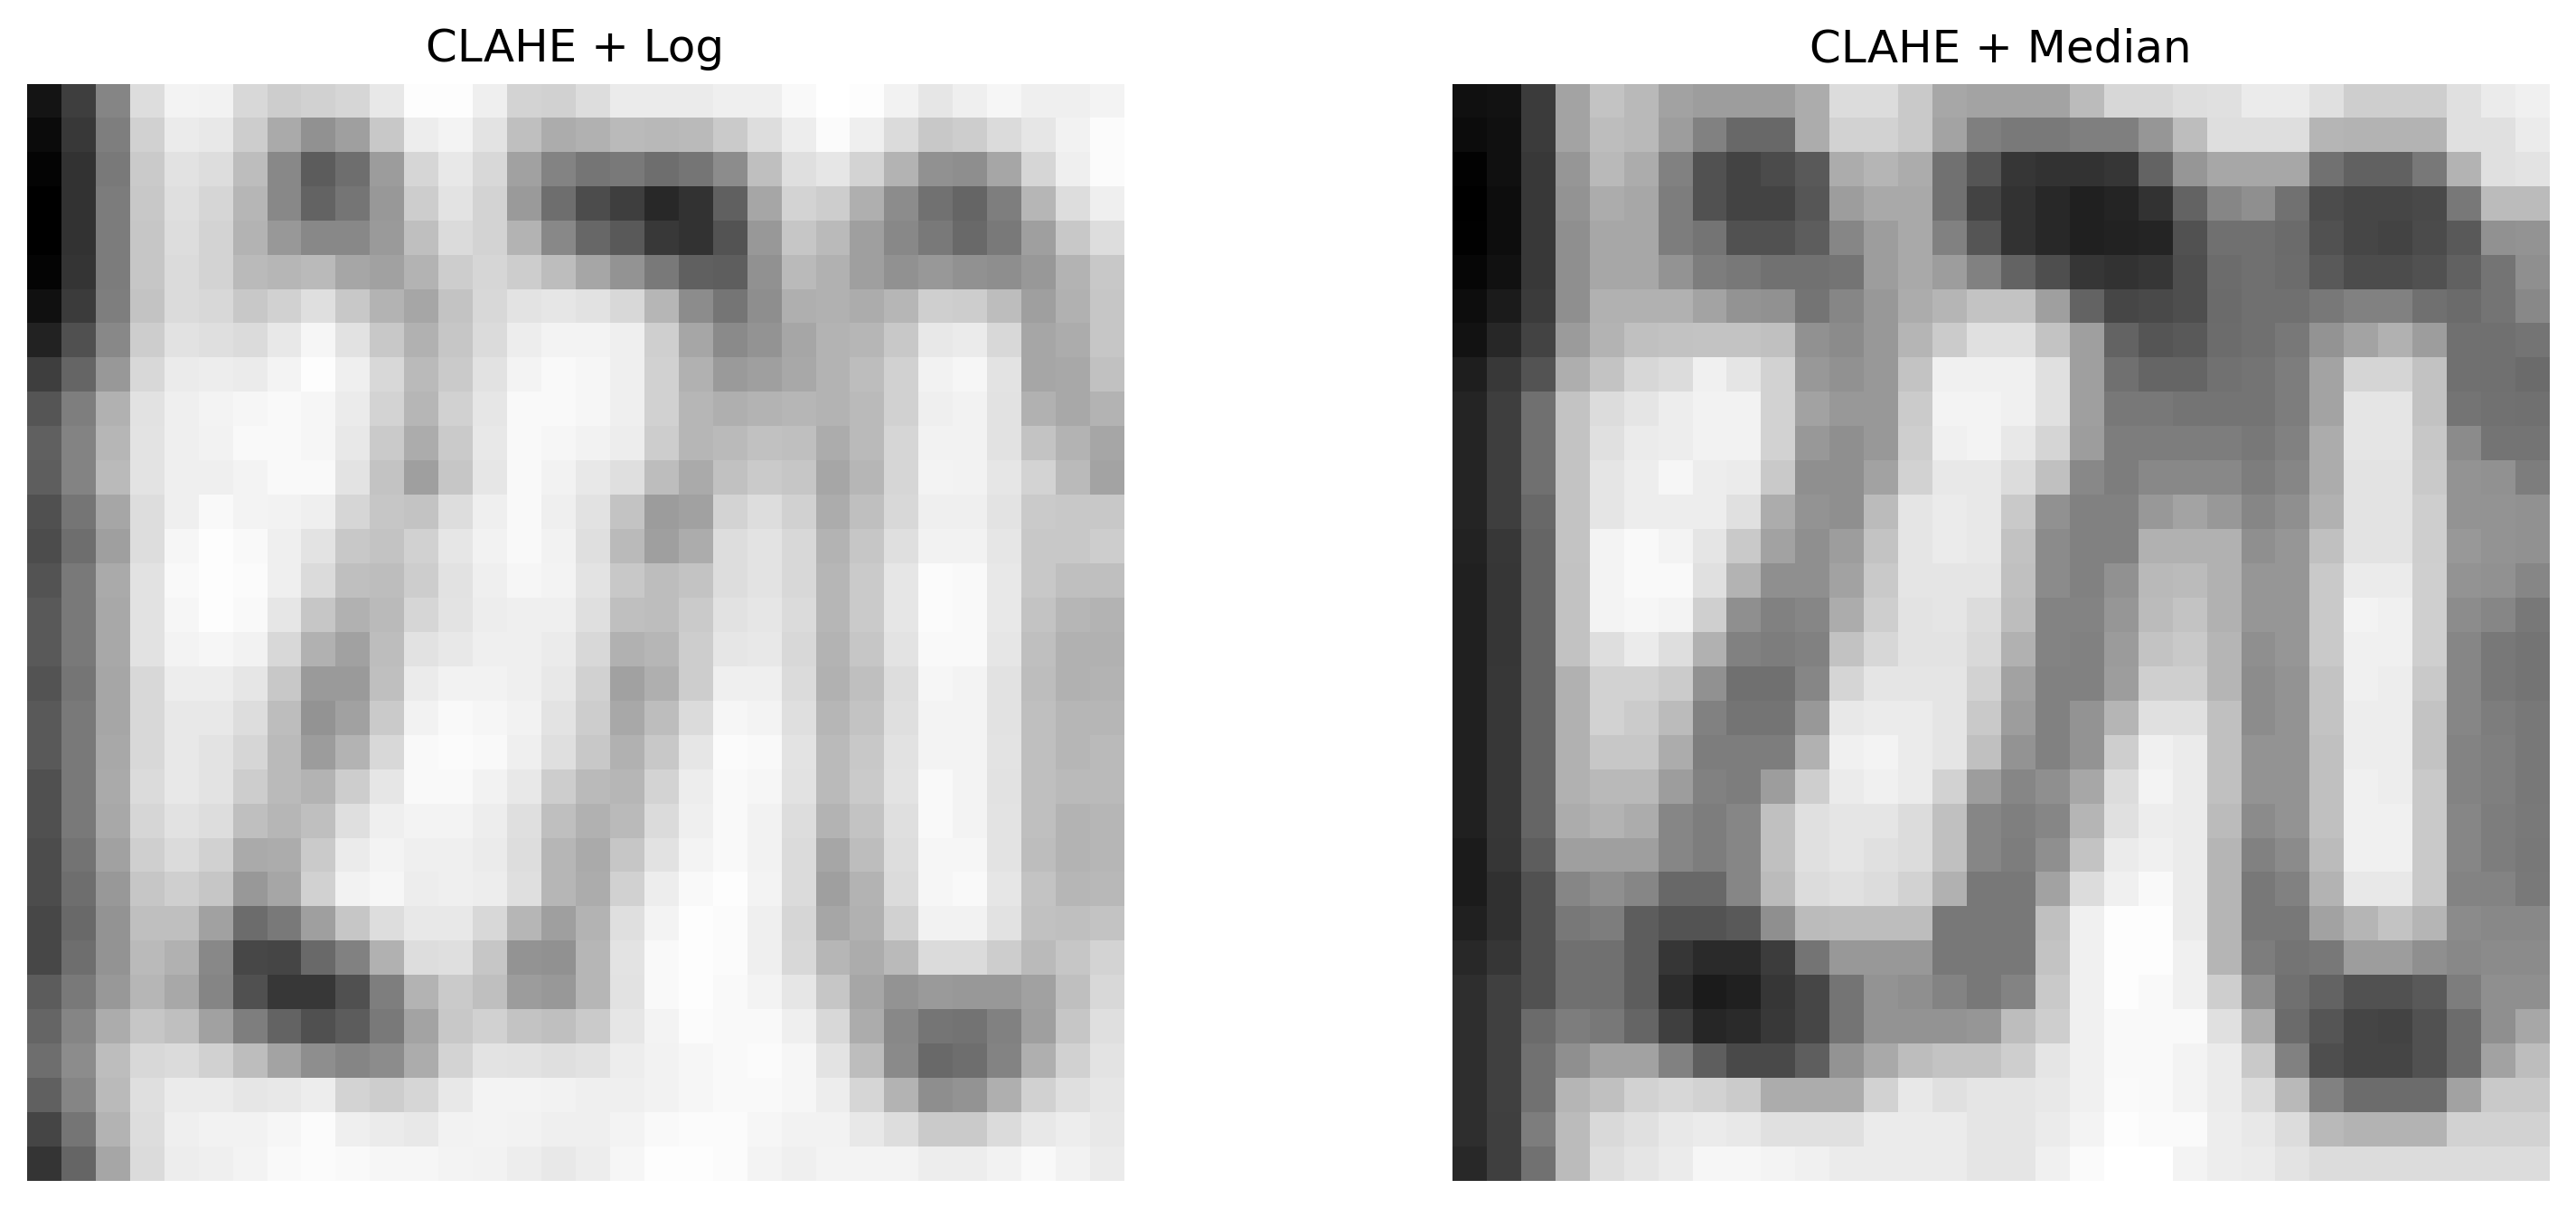
\includegraphics[width=\linewidth]{figures/row_3_images.png}
        \caption{Transformaciones Logarítmicas y Mediana a imagen CLAHE}
        \label{fig:row_3}
\end{figure}

\begin{figure}[H]
        \centering
        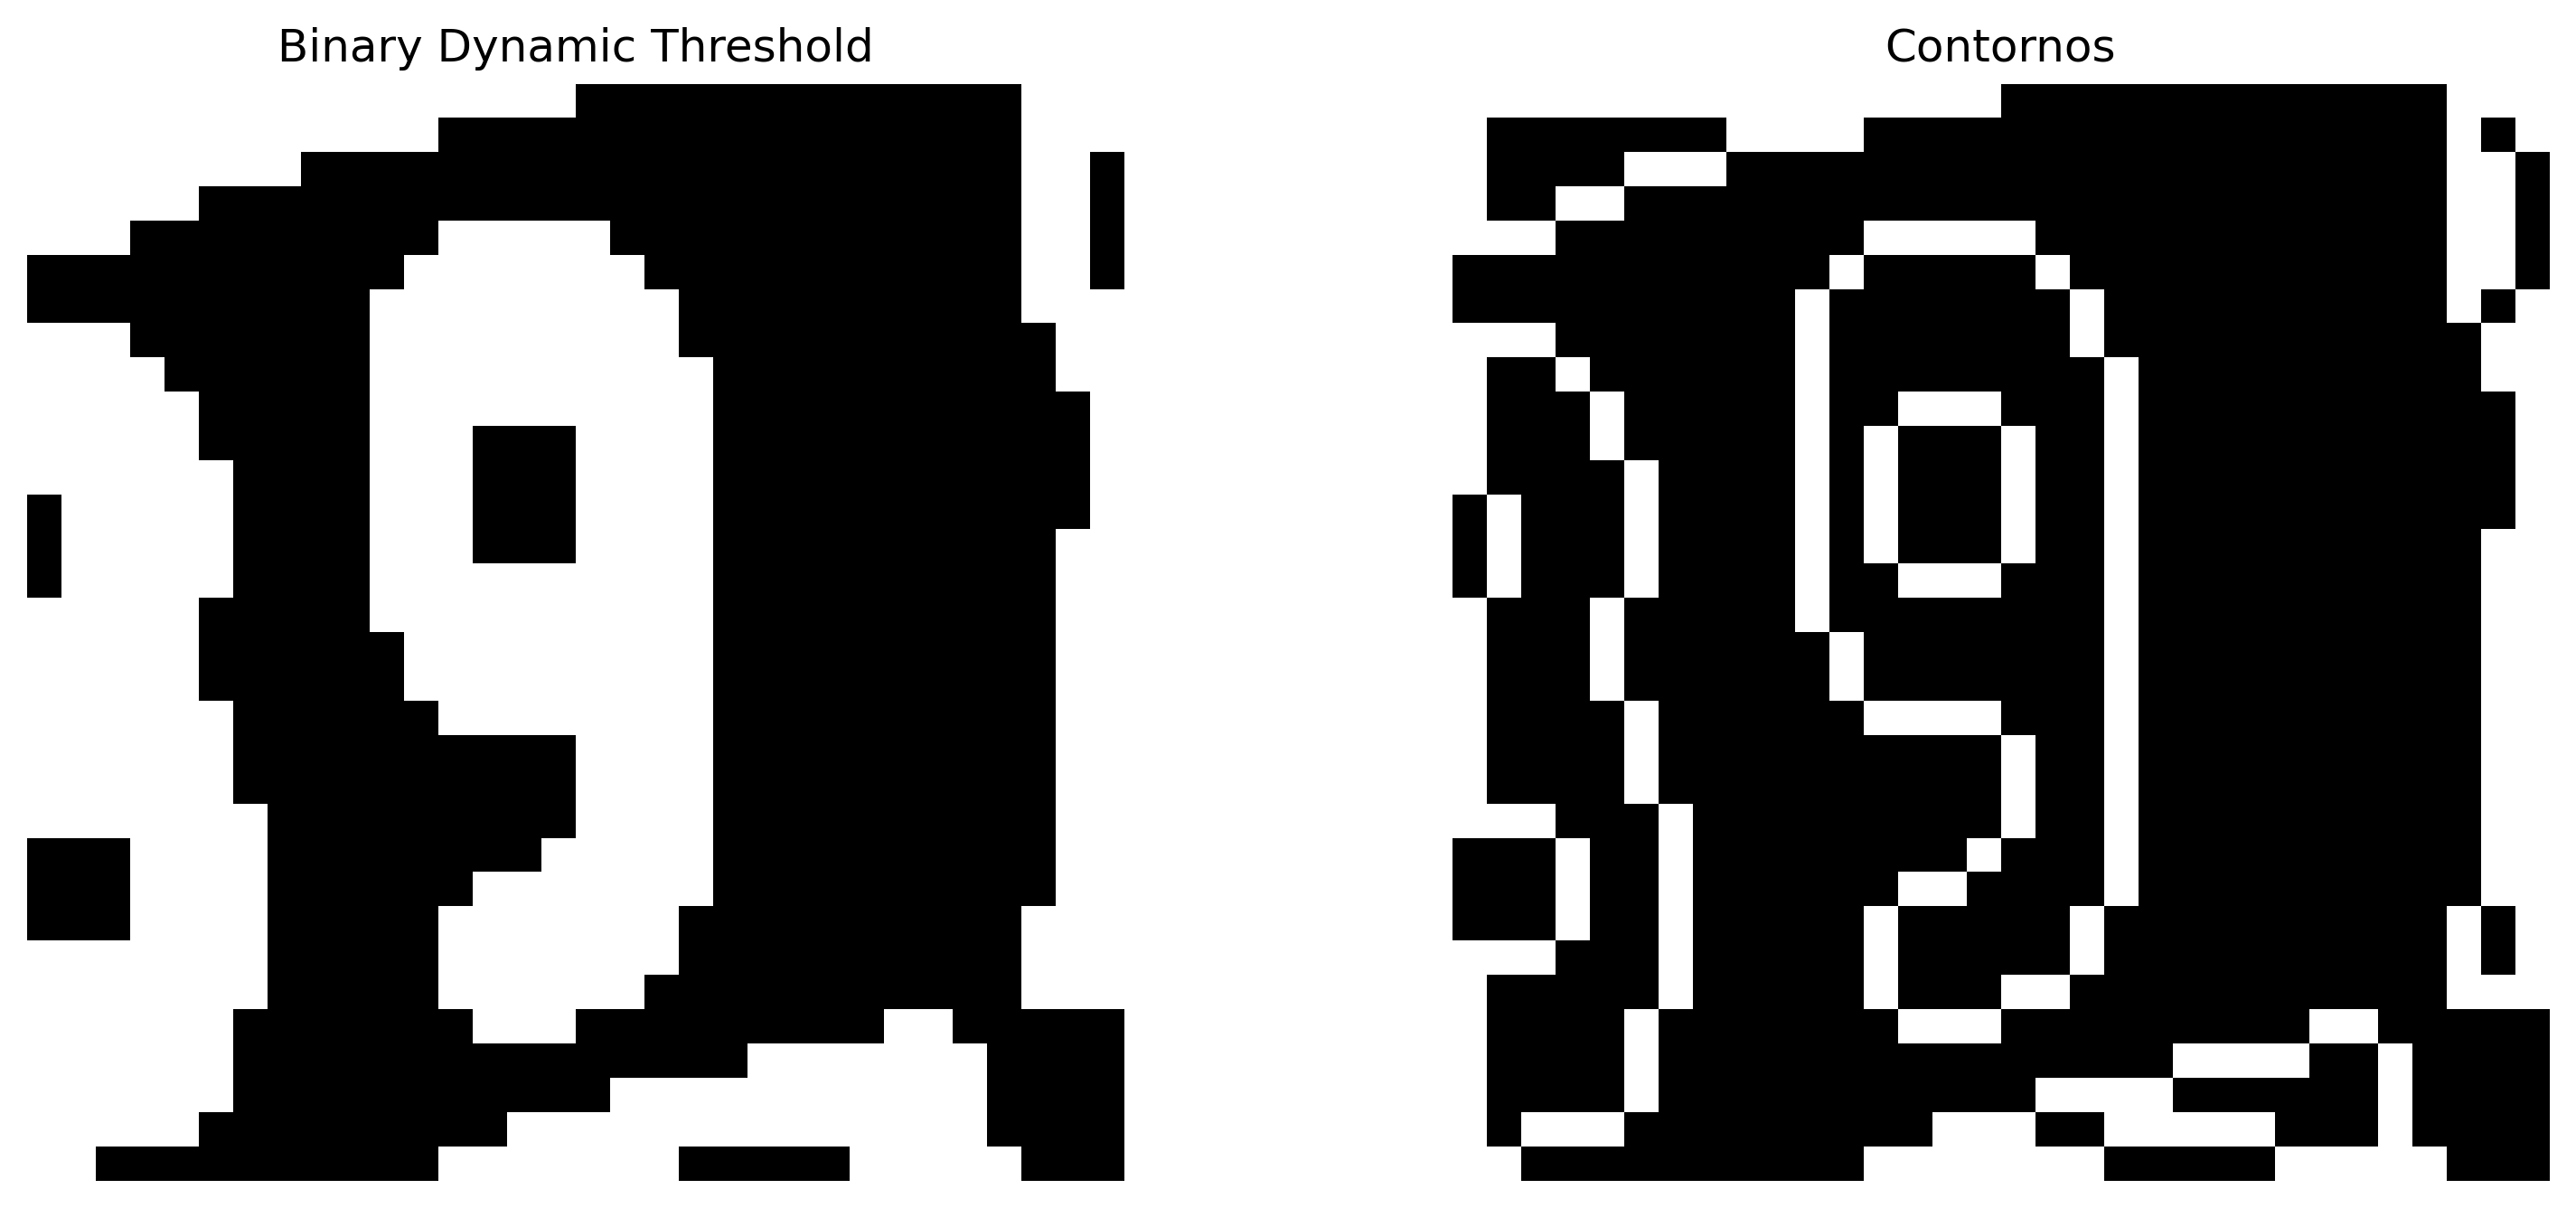
\includegraphics[width=\linewidth]{figures/row_4_images.png}
        \caption{Binary Dynamic Threshold y extracción de contornos}
        \label{fig:row_4}
\end{figure}

\begin{figure}[H]
        \centering
        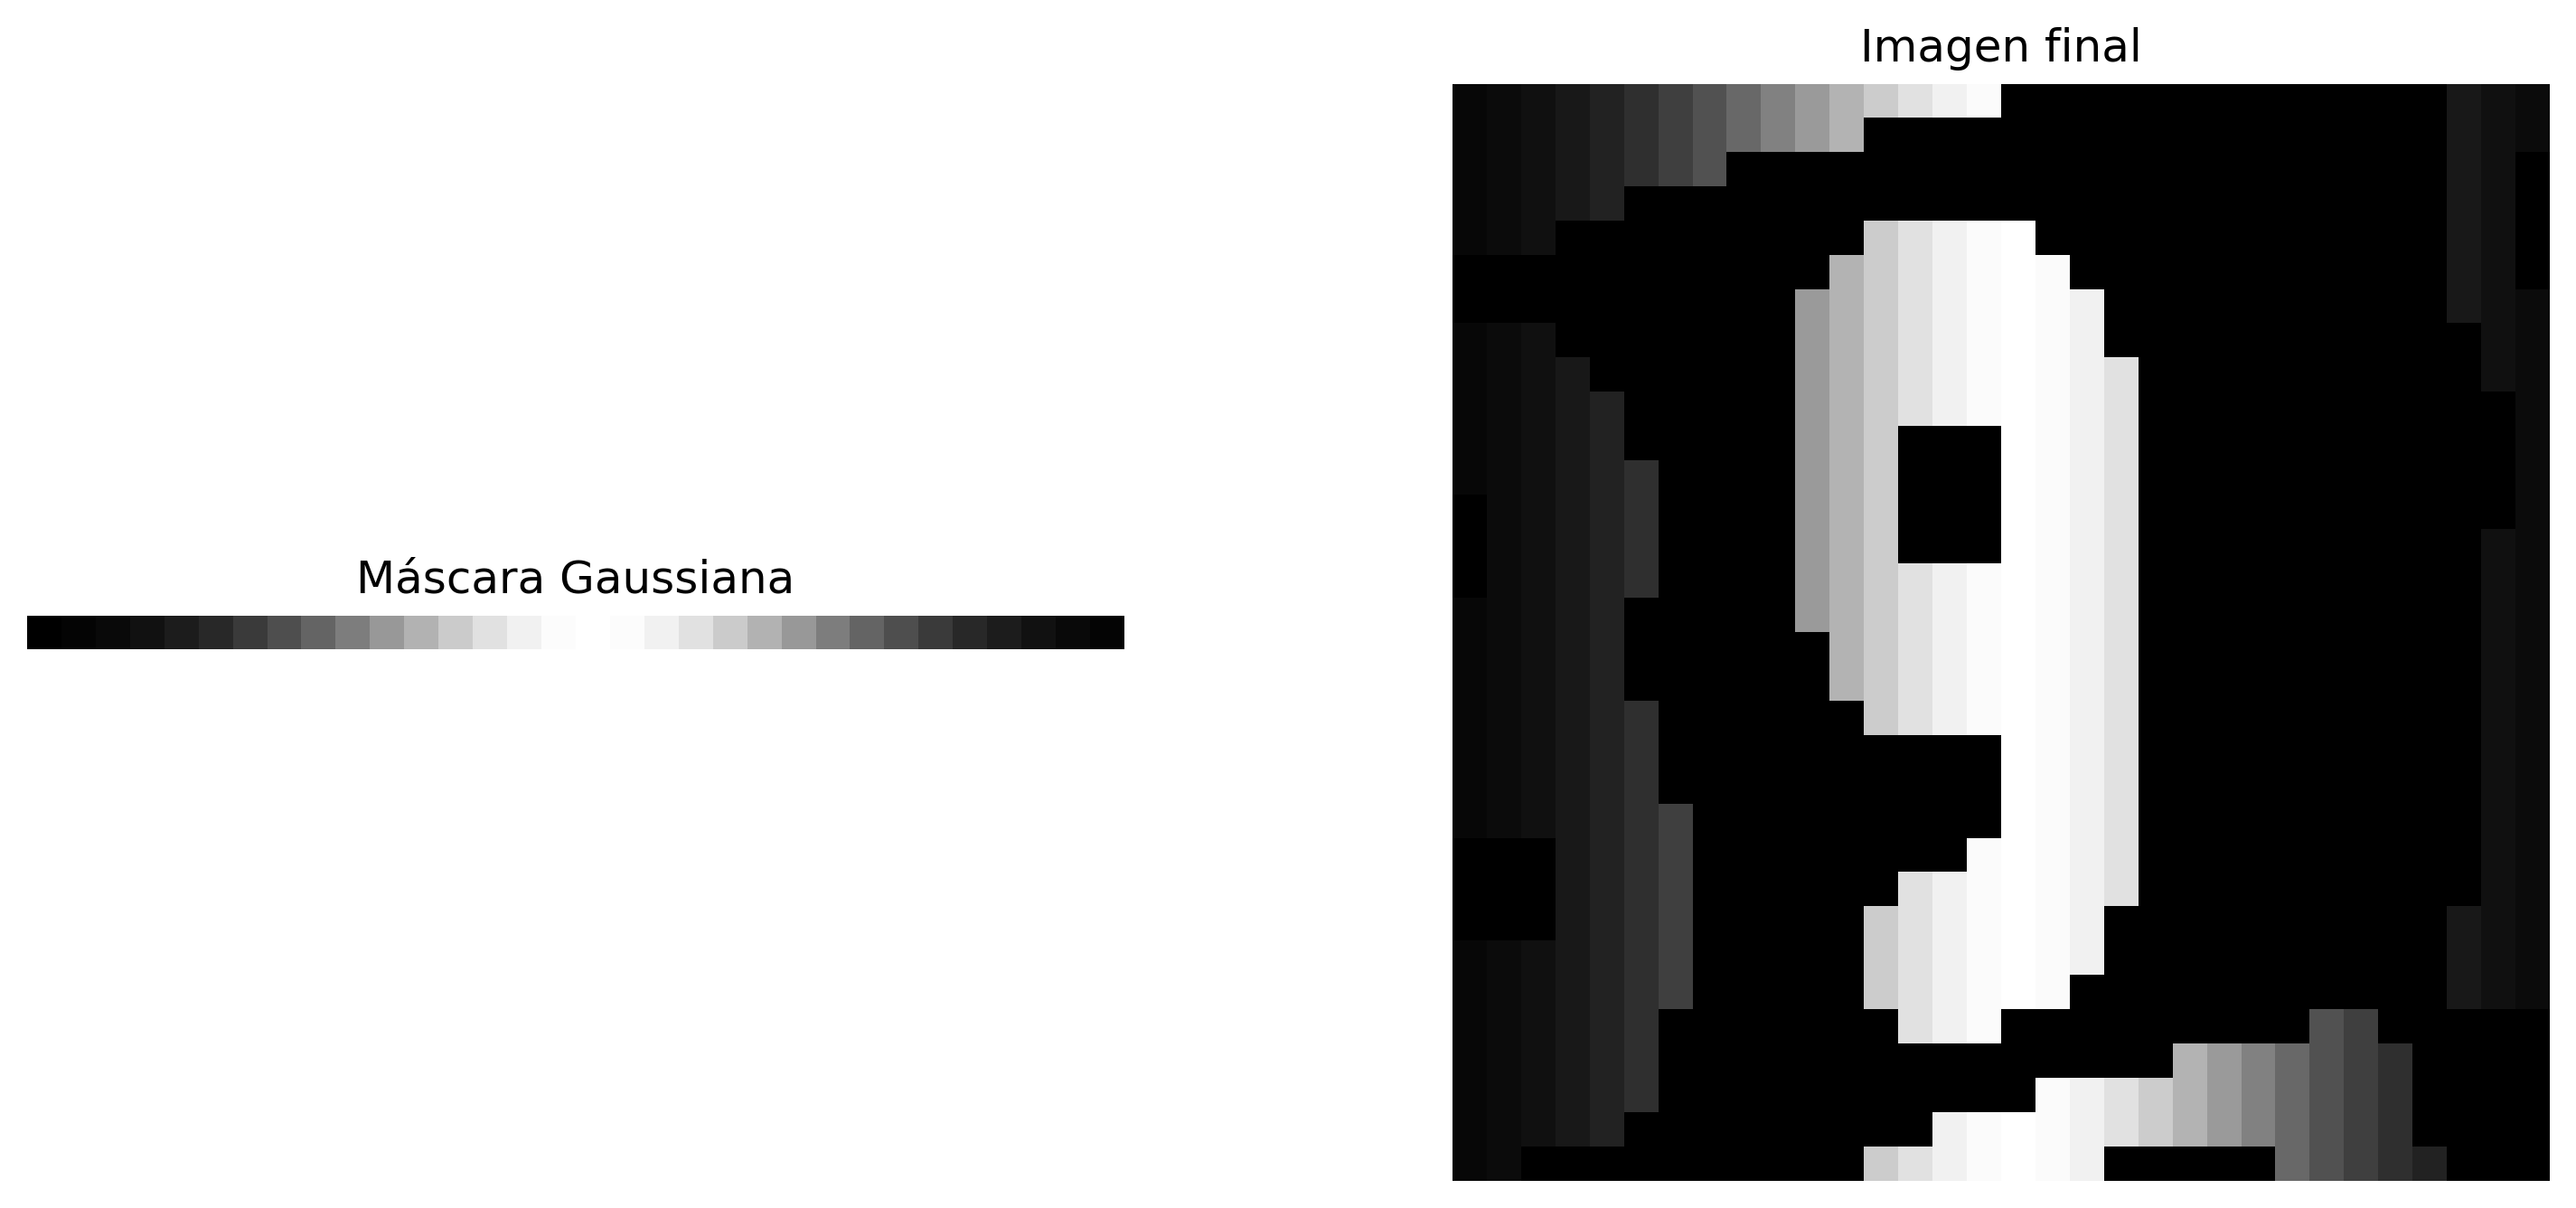
\includegraphics[width=\linewidth]{figures/row_5_images.png}
        \caption{Filtro Gaussiano}
        \label{fig:row_5}
\end{figure}

\subsection{Selección de modelos}
En este primer avance se selecciona un clasificador SGDClassifier de scikit-learn.\cite{scikit-learn_sgdclassifier} La utilización se describe en la siguiente sección de Cross-Validation. Para continuar el ejercicio de apredizaje también se utiliza el modelo de descomposición PCA de scikit-learn.\cite{scikit-learn_pca} 

\subsubsection{PCA}
Una vez pre-procesados los datos, podemos alimentarlos al modelo PCA.

\begin{lstlisting}[language=Python]
from sklearn.decomposition import PCA

pca = PCA(n_components=2)
X_pca = pca.fit_transform(X_train)
\end{lstlisting}

\begin{figure}[H]
        \centering
        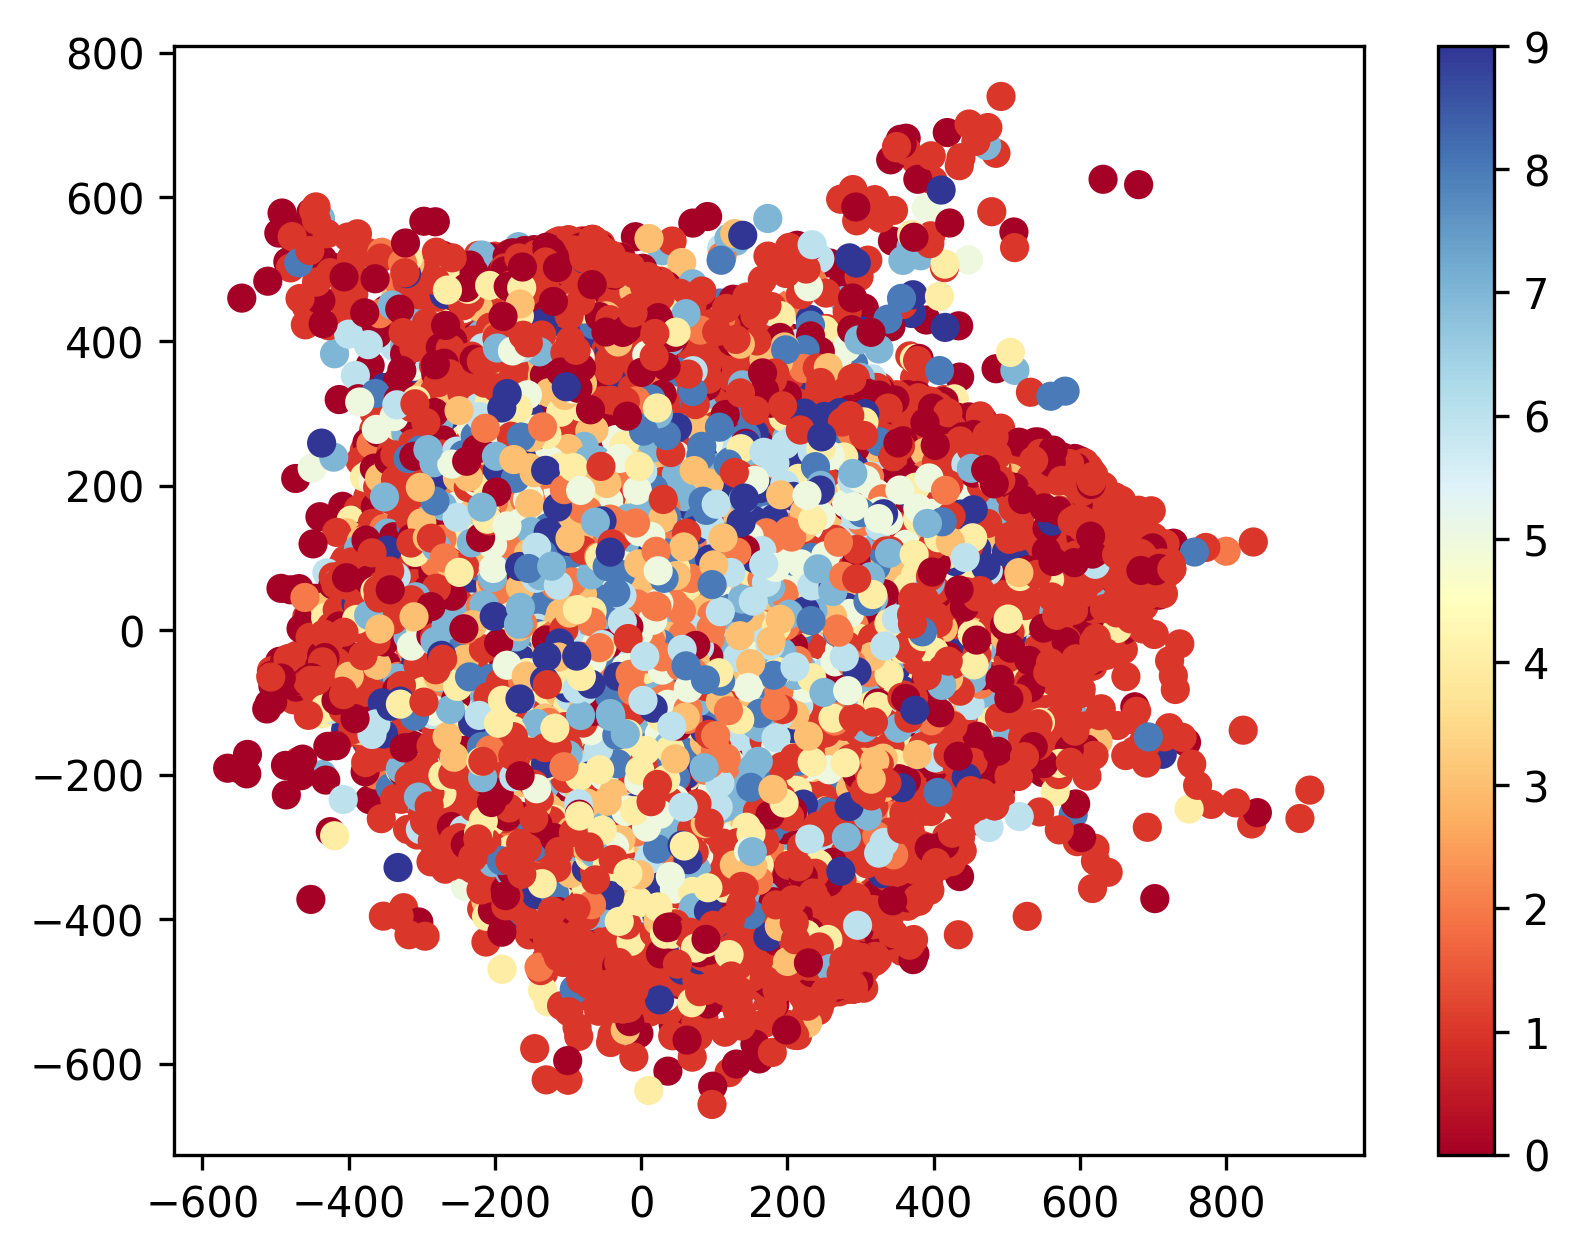
\includegraphics[width=\linewidth]{figures/pca.png}
        \caption{PCA}
        \label{fig:pca}
\end{figure}

\subsection{Cross-Validation}
Debido a la variedad de hiperparámetros y los posibles valores, es importante explorar con diferentes combinaciones para aproximarse a valores ideales. En este ejercicio utilizamos GridSearchCV\cite{scikit-learn_gridsearchcv} combinado con SGDClassifier, ambos de scikit. Se indicaron 2 diferentes funciones de pérdida: hinge y log. Se terminó usando hinge ya que la función de pérdida log no lograba converger. Para este caso se acudirá con el profesor para indagar más al respecto.

\begin{lstlisting}[language=Python]
from sklearn.model_selection import GridSearchCV

parameters = {
        'alpha'    : [0.001, 0.01 ,0.1],
        'max_iter' : [1000, 2000],
        'loss'     : ["hinge", "log"]
}

model = SGDClassifier()
gridsearch = GridSearchCV(estimator=model,
                          param_grid=parameters,
                          n_jobs=3)
gridsearch.fit(X_train, Y_train)
gridsearch.best_params_
> gridsearch.best_params_
{'alpha': 0.1, 'loss': 'hinge', 'max_iter': 1000}
\end{lstlisting}

\subsection{Entrenamiento y Validación}
Una vez ejecutado el paso de Cross-Validation, se cuenta con un conjunto de hiperparámetros que pueden usarse para entrenar y obtener el score de nuestro modelo con los datos pre-procesados. Para esto, se declara un modelo SGDClassifier, como se mencionaba en las secciones anteriores, con los mejores parámetros encontrados por GridSearchCV. Se logró un score final de \textbf{0.33}

\begin{lstlisting}[language=Python]
model = SGDClassifier(
         alpha=best_params['alpha'],
         max_iter=best_params['max_iter'],
         loss=best_params['loss']
        )

model.fit(X_train, Y_train)
model.score(X_test, Y_test)
> 0.33320528580208975
\end{lstlisting}

\section{Conclusiones}

\subsection{Preprocesamiento y Feature Engineering}
Se propone una serie de pasos para transformar de distintas formas cada muestra del dataset. Visualmente y en varios ejemplos se observa cómo cada proceso modifica la información y podría permitir una extracción o representación más concisa del objetivo final. Sin embargo, debido al bajo rendimiento del modelo, podría ser valioso experimentar con otros pasos o realizar Cross-Validation en nuestro proceso de transformación, ya que existen diferentes hiperparámetros que afectan los filtros o funciones de Preprocesamiento. Si bien la imagen final preprocesada puede ser distringuible para un humano al observar los bordes, esto no asegura que un modelo predictivo encuentre relación y logre generalizar con esta información. Ese necesario explorar e investigar más en este aspecto.

\subsection{PCA}
Al aplicar la descomposición PCA obtenemos un resultado visual que no muestra grupos muy definidos, a comparacion de ejemplos con el dataset MNIST, esto podría sugerir que los datos no cuentan con el suficiente preprocesamiento o correcto Feature Engineering para poder clasificar o agrupar. Se espera que después de consultar con el profesor se cuente con más claridad sobre las transformaciones que se usan en este trabajo para confirmar si son de utilidad.

\subsection{Cross-Validation}
En estos ejemplos se intentaron muy pocas combinaciones de hiperparámetros para favorecer rápidos tiempos de ejecución. El hecho de no poder converger con la función de pérdida "log" puede indicar un problema en los valores para el espacio de búsqueda o en nuestro flujo de preprocesamiento. La selección de modelos es limitada a SGDClassifier, pero se reconoce que podría usarse una opción más adecuada para reconocimiento de imágenes. Se buscará continuar explorando otros modelos después de consultar con el profesor.

\subsection{Entrenamiento y Validación}
Se logra observar bajo score \textbf{(0.33)}. Esto sugiere que es importante revisar a detalle los procesos que estamos realizando. Para el siguiente trabajo se identifican estas áreas:
\begin{itemize}
        \item Revisión de Feature Engineering y búsqueda de hiperparámetros con GridSearchCV
        \item Creación de pipeline usando los módulos de scikit\cite{scikit-learn_pipeline}
        \item Exploración de modelos más allá de SGDClassifier
        \item Expandir rango de valores para GridSearchCV
\end{itemize}

Una vez se consulten de forma minuciosa estos resultados con el profesor, se espera observar una mejora considerable en este ejercicio de machine learning.
% if have a single appendix:
%\appendix[Proof of the Zonklar Equations]
% or
%\appendix  % for no appendix heading
% do not use \section anymore after \appendix, only \section*
% is possibly needed

% use appendices with more than one appendix
% then use \section to start each appendix
% you must declare a \section before using any
% \subsection or using \label (\appendices by itself
% starts a section numbered zero.)
%


\printbibliography
\end{document}


